\documentclass[]{article}
%Busca la linea que pone /tableofcontents y empieza a escribir debajo de cada sección.
%Te explico para qué es cada cosa que sea medio relevante:
\usepackage{amsmath}
\usepackage{amssymb}
\usepackage{verbatim} %con verbatim escribes bloques de texto con letra mono.
\usepackage{graphicx} %para insertar imagenes, cuando meta yo una usa el codigo de ejemplo
\usepackage{listings}
\usepackage{fullpage}
\usepackage{color}
\usepackage{fancyvrb}
\usepackage[spanish]{babel}
\usepackage[utf8]{inputenc} %Para usar acentos directamente en latex
\usepackage{hyperref} %Para que el indice tenga hiperenlaces y si quieres poner los tuyos
\hypersetup{%
	pdfborder = {0 0 0}
}

\definecolor{mygreen}{rgb}{0,0.6,0}
\definecolor{mygray}{rgb}{0.5,0.5,0.5}
\definecolor{mymauve}{rgb}{0.58,0,0.82}

%Para insertar código: crea un recuadro con texto mono y lineas enumeradas. Puedes referenciar un fichero y no copiar y pegar aquí.
\lstset{ %
	backgroundcolor=\color{white},   % chohttp://xdxd.com/ose the background color; you must add \usepackage{color} or \usepackage{xcolor}
	basicstyle=\footnotesize,        % the size of the fonts that are used for the code
	breakatwhitespace=false,         % sets if automatic breaks should only happen at whitespace
	breaklines=true,                 % sets automatic line breaking
	captionpos=b,                    % sets the caption-position to bottom
	commentstyle=\color{mygreen},    % comment style
	frame=single,                    % adds a frame around the code
	keepspaces=true,                 % keeps spaces in text, useful for keeping indentation of code (possibly needs columns=flexible)
	numbers=left,                    % where to put the line-numbers; possible values are (none, left, right)
	numbersep=5pt,                   % how far the line-numbers are from the code
	numberstyle=\tiny\color{mygray}, % the style that is used for the line-numbers
	rulecolor=\color{black},         % if not set, the frame-color may be changed on line-breaks within not-black text (e.g. comments (green here))
	showspaces=false,                % show spaces everywhere adding particular underscores; it overrides 'showstringspaces'
	showstringspaces=false,          % underline spaces within strings only
	showtabs=false,                  % show tabs within strings adding particular underscores
	stepnumber=1,                    % the step between two line-numbers. If it's 1, each line will be numbered
	stringstyle=\color{mymauve},     % string literal style
	tabsize=4,
	inputencoding=utf8,
	title=\lstname                   % show the filename of files included with \lstinputlisting; also try caption instead of title
}



\title{Servicios Telemáticos Avanzados\\ENERO 2016}
\author{José Luis Cánovas Sánchez - 48636907A\\Ezequiel Santamaría Navarro - 20096517Z}

\begin{document}

\maketitle

\begin{abstract}
En esta memoria se describen el despliegue y configuración de las topologías y servicios de dos organizaciones, tanto de manera ideal, donde disponemos de suficientes recursos, como la implementación en los laboratorios de prácticas.
\end{abstract}

\tableofcontents


\section{Introducción}

Como grupo 3 de prácticas, desplegaremos las organizaciones 31 y 32. En la descripción de cada servicio desplegado indicaremos en los párrafos iniciales el despliegue que haríamos en una situación real y con recursos, es decir, donde tuviéramos un router por organización, más de una o dos máquinas físicas, varios switches, puntos de acceso, firewall, usuarios, clientes, etc. A continuación, la descripción del despliegue que hemos realizado y configurado en los ordenadores de prácticas y sus equivalente máquinas virtuales cuando no había acceso al laboratorio 2.7.

Primero describimos la topología de las organizaciones, segundo el despliegue de la gestión por SNMP y Nagios, a continuación el servicio VoIP desplegado con Asterisk, finalmente entre los servicios, Owncloud haciendo uso de LDAP. No puede faltar la seguridad de la organización, con iptables, y la certificación de Owncloud por medio de nuestra propia jerarquía de certificados.

El trabajo en grupo ha consistido en que ambos hemos desarrollado y configurado todo conjuntamente, no hay un reparto en el que un miembro se encarga de SNMP, otro de VoIP, otro de Owncloud, etc., sino que ente los dos avanzamos en cada servicio conjuntamente, lo que se refleja en nuestro repositorio git de GitHub, donde cada semana hay como mínimo un par de commits. Es verdad que hay ocasiones donde no podemos quedar en el laboratorio y tampoco en la casa de uno de los dos, en esos casos uno solo avanza por su cuenta escribiendo el código o probando el servicio, pero la decisión previa de qué se va a modificar o escribir, el diseño de la parte del servicio que uno solo va a implementar, se hace en común, normalmente por chats como Telegram. En caso de imprevistos que sobrepasaran a uno sólo, se hacía un commit y hasta que se hablase el problema no se continuaba, pero eran los menos.

\begin{center}
	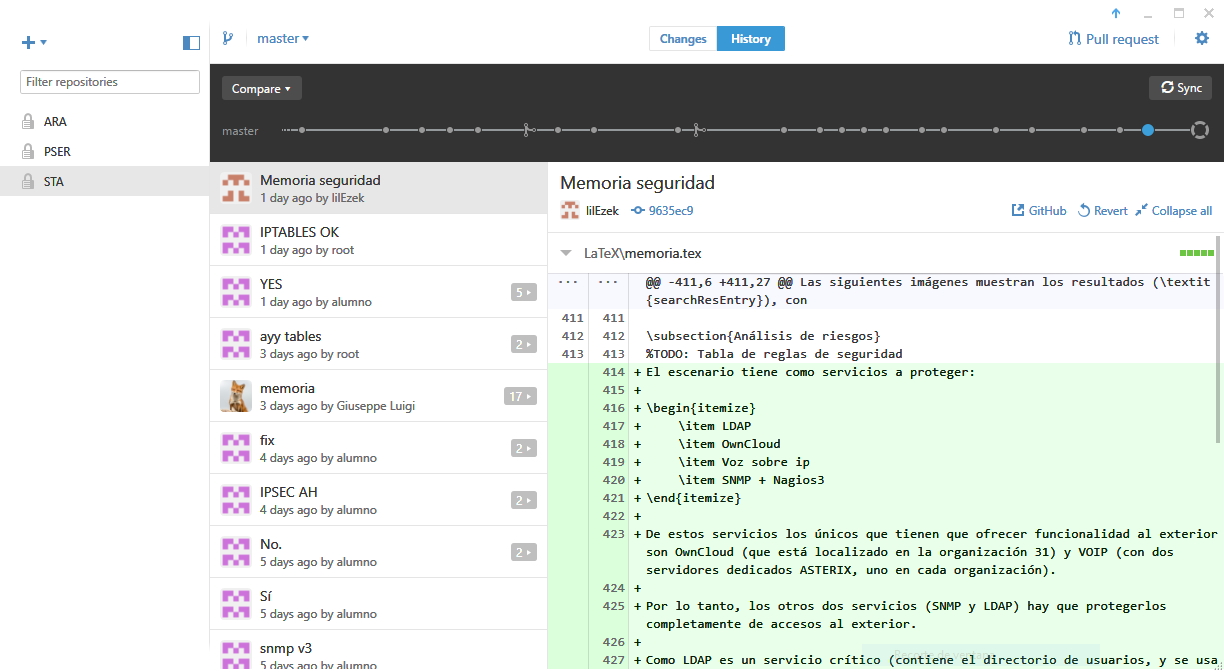
\includegraphics[scale=0.5]{images/git.PNG}
\end{center}


\section{Topología}

En esta sección describimos la forma en la que se van a desplegar los servicios y como estarán
conectados entre sí.

\subsection{Solución ideal}

Imaginemos que estamos en una empresa real con recursos suficientes. Nuestro diseño de la topología de cada organización se basaría en una red DMZ aislada por un firewall donde dispondríamos los servidores de cada servicio, Owncloud, centralita de voz, manejador SNMP, LDAP, etc. También habría una subred dentro de la organización donde se conectarían los usuarios y empleados, por medio de switches y puntos de acceso inalámbricos.

La red de servidores tendría una máquina física para cada servicio, para asegurar a cada uno los recursos mínimos que necesite y evitar que ante el fallo de uno, puedan caer otros servicios. Para la gestión de dispositivos por SNMP habrá una VLAN específica para este tráfico, que al incluir al router, se debe extremar la seguridad. El tráfico VoIP pasaría siempre por la centralita, para controlar tanto las llamadas realizadas como el tráfico de voz IP que entra y sale de la organización por los mismos puertos y equipo servidor. El firewall permitiría el tráfico saliente de la subred de empleados, pero nunca el entrante desde internet, sólo desde la red DMZ. Así, la red DMZ no podría iniciar comunicaciones excepto las básicas para su funcionamiento como actualizar las listas CRL, llamadas VoIP, etc., restringiendo en las reglas qué servidor en concreto tiene dichos permisos. El tráfico entrante desde fuera se reenviaría siempre a la DMZ, si coincide con el tipo de mensajes que la IP destino espera por sus tipo de servicio (peticiones HTTP/S sólo si van dirigidas al servidor Owncloud, por ejemplo).

En la \autoref{fig:topoideal} se muestra el diagrama de nuestra topología.

\begin{figure}[h]
	\centering
	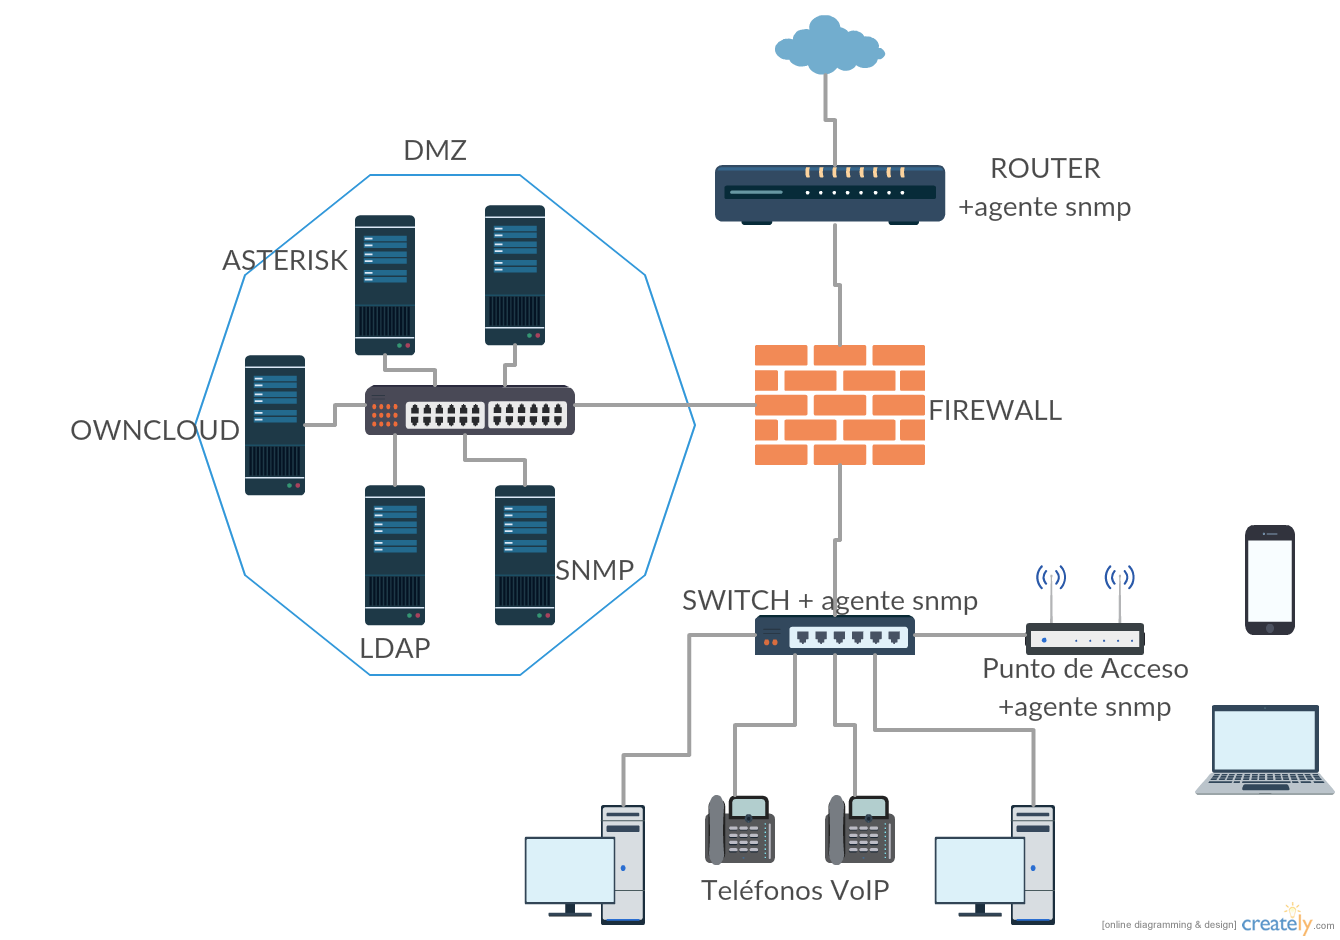
\includegraphics[scale=0.35]{images/topoideal.png}
	\caption{Topología ideal}
	\label{fig:topoideal}
\end{figure}

\subsection{Dispositivos disponibles}

Tenemos para las pruebas y el desarrollo de la práctica, las siguientes herramientas hardware:

\begin{itemize}

	\item Un \textbf{switch} con VLAN y 5 puertos.
	\item Un ordenador que actúa de \textbf{enrutador}, con dos puertos ethernet, uno de ellos con configuración VLAN.
	\item Un \textbf{punto de acceso} WiFi para el acceso a la red.
	\item Un \textbf{iPhone} y un \textbf{portátil Mac}, útiles para probar VOIP con wifi.
	\item Dos ordenadores que actúan como \textbf{organizaciones} 31 y 32.
	\item Dos ordenadores más para simular \textbf{clientes} haciendo peticiones.

\end{itemize}




\subsection{Topología desplegada}

En cuanto a la topología física real, disponemos en el laboratorio de 3 torres, 5 puertos del switch CISCO y un punto de acceso wifi configurado para la organización 31. La conexión de una de las torres como router y las otras dos como equipos de cada organización ya se explica en los boletines de prácticas.

A partir de esa configuración básica, configuramos las dos organizaciones de manera casi simétrica: en la \textbf{máquina física} de cada organización se ejecutarán \textbf{todos los servicios}, es decir, del diseño lógico ideal donde cada servicio tiene una máquina física para él solo, ahora todos los servicios conviven en la misma máquina física. Decidimos usar un servidor físico porque la cantidad de servicios proporcionados por la organización no son tan pesados como \textbf{carga de trabajo} conjunta para una única máquina, como lo pueda ser tener \textbf{varios} servidores como \textbf{máquinas virtuales} en la misma torre del laboratorio.

Ahora bien, por el modo en que programamos la instalación de servicios, nos es muy fácil portarlos desde una máquina física a varias, cambiando las configuraciones de la IP de cada máquina.

En la \autoref{fig:topofisica} vemos el diagrama de la topología física, donde tenemos el ordenador que hace de router, los otros dos ordenadores del laboratorio que actuarán de servidores, el punto de acceso donde usamos nuestros móviles y portátiles personales, y la posibilidad de usar otra torre del laboratorio como cliente.


\begin{figure}[h!]
	\caption{Topología física}
	\centering
		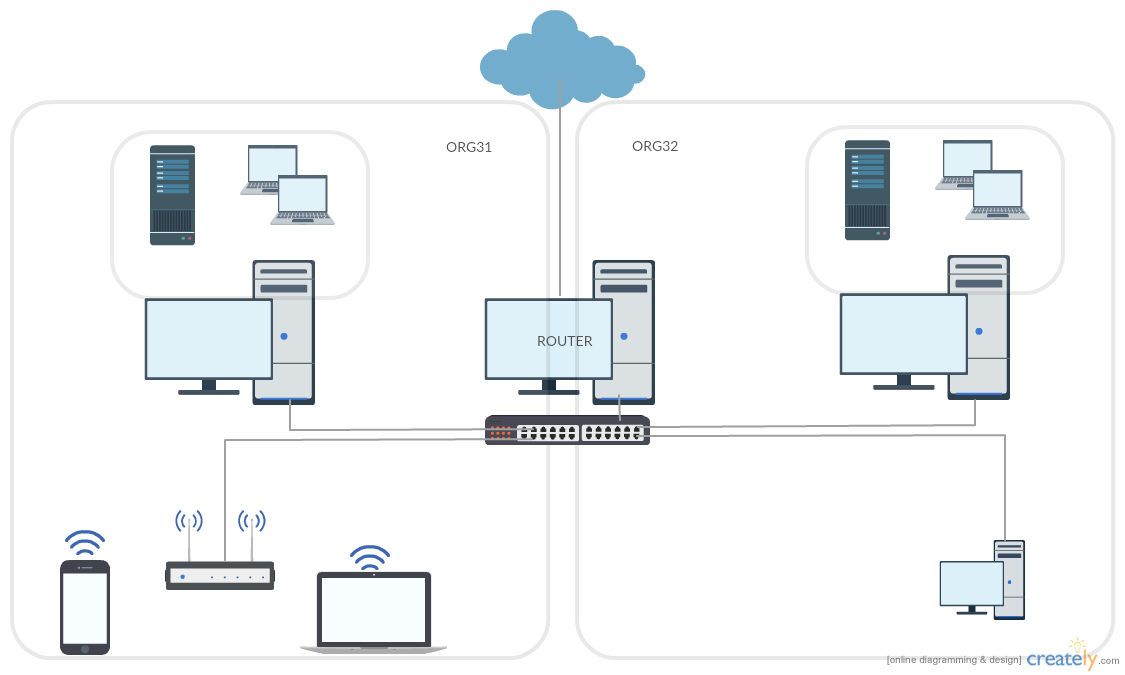
\includegraphics[scale=0.35]{images/TopologiaFisica}
	\label{fig:topofisica}
\end{figure}




\section{Configuración automatizada de los equipos}

Para la configuración de los dispositivos utilizamos herramientas Makefile, y scripts escritos en bash y python, de manera que desplegar los servicios y la topología en un dispositivo esté automatizado, llegando a tal punto que en la instalación sólo haría falta intervenir para escribir la contraseña de la base de datos de Owncloud y pulsar Intro en alguna instalación. No nos apoyamos en una máquina virtual que vayamos configurando a lo largo de las prácticas llevándola de un lado a otro, y por lo general, usamos máquinas virtuales con una instantánea \textit{limpia}.
\\

Usamos una estructura de directorios basada en el hardware a configurar. Es decir, en el ordenador que hace de router ejecutamos un Makefile que está en el directorio ROUTER; para la máquina servidor de la organización 31, la carpeta SERVER contiene su Makefile correspondiente; etc.

\begin{BVerbatim}
ROUTER
	SNMP
	Makefile
	network
	test
	iptables
ORG1
	SERVER
		CERTS
		IPSEC
		LDAP
		OWNCLOUD
		SNMP
			NAGIOS
		VOIP
		Makefile
		network
		test
		
\end{BVerbatim}

\hfill




\section{Servicios}

\subsection{Enrutamiento}

Del enrutamiento se encarga el PC que hace de router. La configuración física se basa en dos puertos Ethernet y VLAN:

\begin{itemize}
	\item Un puerto se usa para conectarse a la red de la UMu, que da conectividad al exterior.
	\item Otro puerto, conectado al \textit{trunk switch vlan} de la organización 31 y 32.
\end{itemize}

La configuración lógica, es decir, la configuración de los interfaces de red es la siguiente:

\lstinputlisting{../ROUTER/network}
%Explicación del fichero: DONE

El script instala el soporte de vlan en el ordenador, desactiva el gestor de redes de ubuntu, copia en \textit{/etc/network/interfaces} la configuración de los puertos ethernet: eth0 conexión a la red UMu con DHCP; eth1.31 y eth1.32 las dos VLAN para el segundo puerto ethernet. A continuación, copia en \textit{/etc/hosts} los nombres correspondientes a las IPs de las máquinas de cada organización, para solventar la falta de un servidor DNS que los registre. Hay máquinas de más de cara a posibles expansiones durante el desarrollo de la práctica. Por último activa el \textit{forwarding} de paquetes y la regla de iptables para actuar como NAT para la subred 192.168.0.0/16, enviando los paquetes por eth0 hacia la red de la UMu.

En las máquinas servidor basta con modificar el fichero \textit{/etc/network/interfaces} para configurar la IP fija 192.168.3i.100 i$ \in \{1,\ 2\} $, pues no tenemos servidor DHCP para autoconfiguración.


\subsection{SNMP}
%DONE

En la topología ideal descrita hemos indicado que habría un servidor dedicado para SNMP. En concreto sería para el manejador, con un acceso por VLAN de gestión desde un ordenador del administrador en la red interna. El resto de servidores, el firewall, el router, los switches y los puntos de acceso inalámbricos tendrían instalados SNMP como agente.

La configuración de cada dispositivo sería:
\begin{itemize}
	\item Todos los dispositivos usarían SNMPv3 y la lectura siempre con autenticación de usuario como mínimo.
	\item El router y firewall, por ser elementos más críticos, además de autenticación, con encriptación, y nunca permisos de escritura.
	\item Los únicos dispositivos con posibilidad de escritura serían los switches y puntos de acceso en la red interna, y añadiendo encriptación.
	\item Los traps (quitando el caso de que no funcionara \textit{monitor}) serían:
		\subitem En los switches, cuando la interfaz donde se conecta un punto de acceso u otro switch esté caída.
		\subitem En los servidores, cuando la interfaz o puerto del servicio que dan, más los básicos como SSH, estén caídos. El trap de la interfaz sólo llegaría si tuviera más de una conectada a la subred.
		\subsubitem En el servicio Owncloud y VoIP cuando el ancho de banda llegue al 80\% de la capacidad máxima, por ser servicios que dependen de buena conexión para una correcta experiencia de uso.
		\subsubitem En Owncloud además, si el espacio de disco duro libre es inferior al 30\%.
\end{itemize}

\hfill

En nuestra topología de prácticas, cada organización tiene un manejador en la máquina física, y como agentes la propia máquina y el router, que al ser también la misma máquina para ambos, en su configuración como agente incluye los \textit{community} de ambas organizaciones.

En cuanto a la seguridad, el router tendrá sólo acceso de lectura con autenticación y cifrado de los mensajes; el servidor de la organización también tendrá permisos de sólo lectura, pero el acceso se relaja a autenticación sin cifrado.

Por problemas descubiertos con los paquetes de SNMP donde la orden \textit{monitor} no funciona, con posible solución la compilación de los paquetes snmp, decidimos instalar en el servidor de la organización 31 Nagios, añadiendo la monitorización de disco y ancho de banda del router, como se explicará en su sección.

\subsubsection{Agentes}
%DONE

El script en los agentes instala los paquetes \textit{snmp}, \textit{snmpd} y \textit{snmp-mibs-downloader} y copia en \textit{/etc/snmp/} los ficheros \textit{snmp.conf} y \textit{snmpd.conf} ya preparados para cada máquina en particular.

En el \textbf{router}, que actúa como agente en las organizaciones 31 y 32, tenemos en \textit{snmpd.conf} el fichero por defecto en la instalación de los paquetes, añadiendo un usuario con autenticación por MD5 y cifrado por DES, donde en el control de acceso se amplía al árbol 1.3.6.1.2.1 para dar acceso a comprobaciones de ancho de banda con los MIBs 1.3.6.1.2.1.2.2.1.2,  1.3.6.1.2.1.2.2.1.10., 1.3.6.1.2.1.2.2.1.16., los cuales usaremos más adelante con Nagios, y define los \textit{community} \textit{sta31} y \textit{sta32}, uno por organización. Los cambios restantes son sobre la información de la máquina modificando los MIBs \textit{sysLocation} y \textit{sysContact}, y finalmente indicando que los traps e informs se envíen a los manejadores de ambas organizaciones. En el caso de haber dos routers, cada uno se comunicaría únicamente con el manejador de su organización.

En el \textbf{servidor}, que actúa también de manejador, la configuración como agente es como en el router, pero el usuario creado sólo tiene autenticación por MD5, sólo hay un nuevo \textit{community}, \textit{sta31}, o \textit{sta32} en la Organización 32.

\subsubsection{Manejador}
%DONE

Como manejadores, los servidores de cada organización añaden al fichero \textit{snmptrapd.conf} las líneas \textit{donotlogtraps 0} y	\textit{authCommunity log,execute sta31} para aceptar los traps de los agentes, cambiando en la Organización 2 el \textit{community} por \textit{sta32}.



\subsubsection{Nagios}
%DONE

Como servicio extra a la gestión de dispositivos en red, y supliendo la falta de \textit{monitor} para poder configurar nuevos traps en los agentes, instalamos Nagios en la Organización 31 para monitorizar el servidor y el router.

Para todos los controles sobre el servidor y la carga de cpu que usa el router, usamos las herramientas que vienen con Nagios por defecto.

Para la consulta del ancho de banda del router, definimos un nuevo comando \textit{check\_bandwidth}, que hace uso de un script bash de los foros de Nagios, modificado por nosotros para que use SNMP sobre la máquina del router. Entre los cambios más importantes, sobre el script original, tenemos que se usaba para consultar máquinas Cisco, cuya nomenclatura de las interfaces no es compatible con las de linux, y el uso de SNMPv3 con el usuario y contraseñas del router. El script además le indica a Nagios si la situación es del alerta o crítica según unos límites pasados por parámetro que indican los flujos de datos límite para el router.

Las órdenes SNMP que usamos son todas \textit{snmpwalk} sobre los MIBs que identifican las interfaces de una máquina y sus propiedades. En la prueba y análisis de trazas vamos a analizar en concreto la orden que pregunta por las interfaces de red disponibles en una máquina.



Para probar que Nagios consigue hacer consultas con éxito nos aprovechamos del servicio Owncloud de la Organización 31, subiendo un fichero de más de 400MB y descargándolo varias veces en la máquina de la Organización 32, por el mismo usuario de Owncloud, de modo que se genera un tráfico de varios megas por segundo entre organizaciones, que claramente debe pasar por el router.

Más abajo se muestran las imágenes de la descarga paralela y de cómo Nagios comprueba los anchos de banda y muestra el mensaje \textit{CRITICAL} al superar los 15Mbit/s puestos como límite, con unos 74Mbit/s.

\begin{center}
	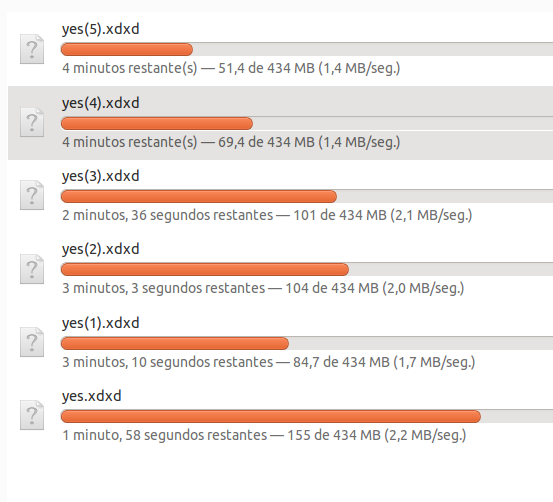
\includegraphics[scale=0.5]{images/snmp/nagios/descargas.png}
\end{center}
\begin{center}
	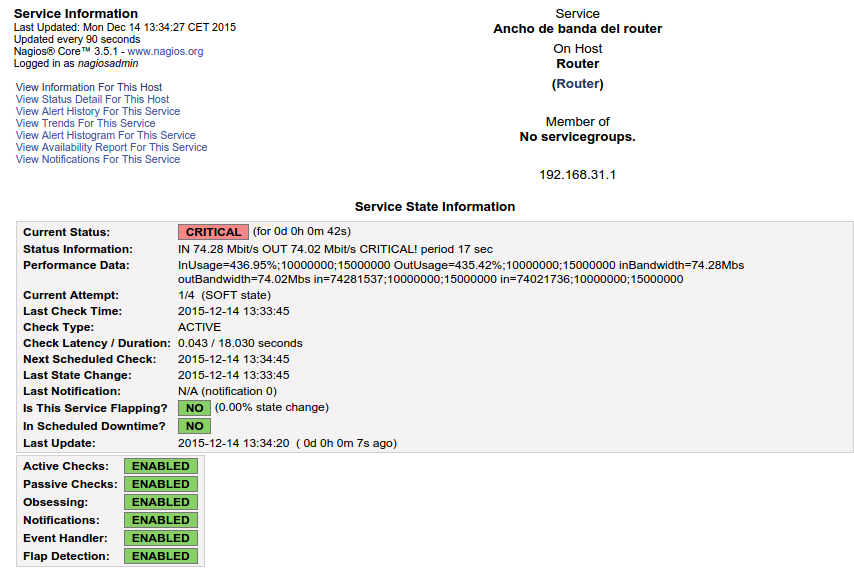
\includegraphics[scale=0.5]{images/snmp/nagios/criticalbandwidth.png}
\end{center}






\subsubsection{Prueba snmpwalk}
%DONE

Para la prueba se ejecutan los siguientes comandos, que consultan el mismo MIB, pero en el primero los mensajes SNMP van cifrados y en el segundo se desactivó temporalmente el cifrado en el agente SNMP del router, dejando sólo autenticación, de modo que se pueden ver el contenido de los paquetes en wireshark.


\begin{Verbatim}[frame=single]
$snmpwalk -v 3 -c sta31 -u router -l authPriv -a MD5 -A 123456789
-x DES -X 123456789 192.168.31.1 1.3.6.1.2.1.2.2.1.2

IF-MIB::ifDescr.1 = STRING: lo
IF-MIB::ifDescr.2 = STRING: eth1
IF-MIB::ifDescr.3 = STRING: eth0
IF-MIB::ifDescr.4 = STRING: eth1.31
IF-MIB::ifDescr.5 = STRING: eth1.32

$snmpwalk -v 3 -c sta31 -u router -l authNoPriv -a MD5 -A 123456789 
192.168.31.1 1.3.6.1.2.1.2.2.1.2

IF-MIB::ifDescr.1 = STRING: lo
IF-MIB::ifDescr.2 = STRING: eth1
IF-MIB::ifDescr.3 = STRING: eth0
IF-MIB::ifDescr.4 = STRING: eth1.31
IF-MIB::ifDescr.5 = STRING: eth1.32
\end{Verbatim}

En ambas capturas los dos primeros mensajes son los mismos: Un primer mensaje \textit{get-request} vacío, sin encriptar, sin autenticar, sin pedir ningún objeto, desde el manejador al agente del router. Después, un mensaje de respuesta \textit{report} con el valor del objeto \textit{usmStatsUnknownEngineIDs}, el cual indica el número de intentos fallidos de paquetes anteriores al referenciar su \textit{snmpEngineID}. Este último paquete además viene con información del Authoritative Engine del router, que es la información que añade en sus paquetes el manejador en los siguientes mensajes.


\begin{center}
	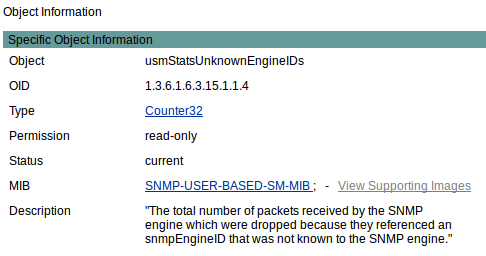
\includegraphics[scale=0.75]{images/snmp/reportMIB.png}
\end{center}

\begin{center}
	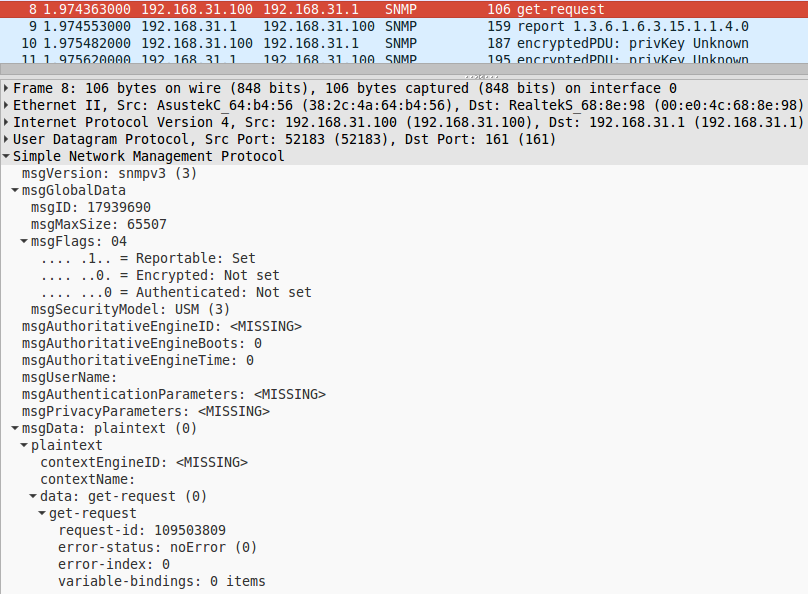
\includegraphics[scale=0.45]{images/snmp/snmp1.png}
	
	\textit{get-request vacío}
\end{center}

\begin{center}
	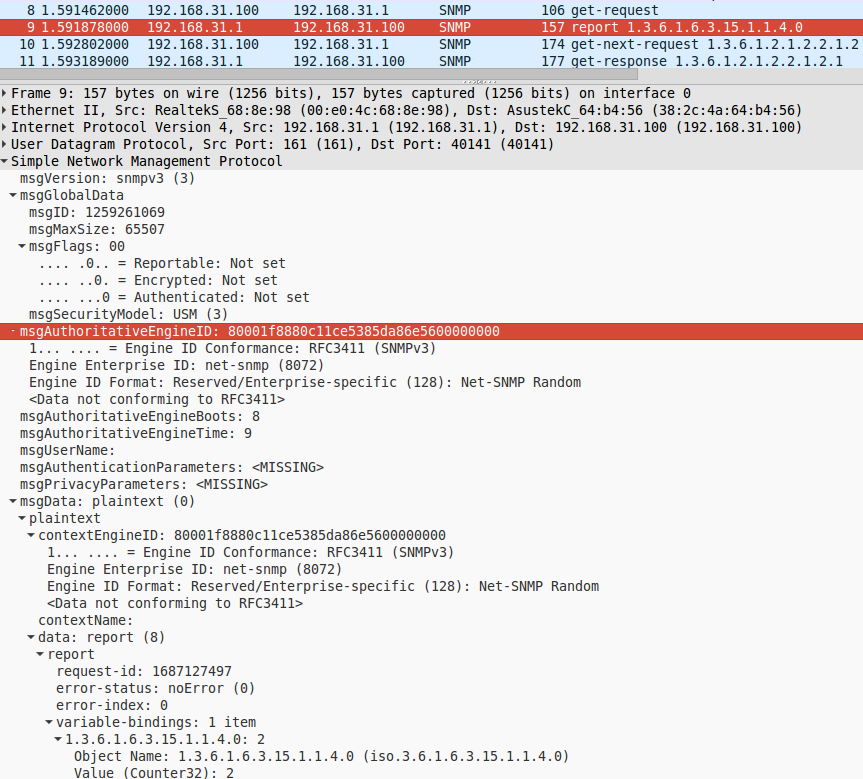
\includegraphics[scale=0.45]{images/snmp/snmp2.png}
	
	\textit{Mensaje report}
\end{center}

En la captura de los mensajes cifrados sólo podemos ver la información del Authoritative Engine ID, el usuario \textit{router} y los parámetros de autenticación y cifrado que acompañan un PDU encriptado. En los paquetes que sólo llevan autenticación, vemos la información anterior y además el PDU con el tipo de mensaje \textit{get-next-request}, el \textit{request-id}, indicadores de error a 0, y la variable pedida.

En nuestro ejemplo pedimos el MIB 1.3.6.1.2.1.2.2.1.2, del cual se obtiene una tabla a recorrer añadiendo .1, .2, etc. al final del MIB:

\begin{center}
	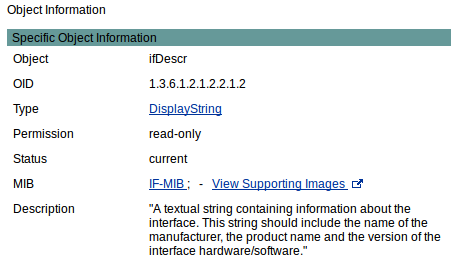
\includegraphics[scale=0.75]{images/snmp/ifDescr.png}
\end{center}

El primer \textit{get-next-request} pide el MIB \textit{ifDescr}, y en la respuesta se le devuelve \textit{ifDescr.1}, el primer descriptor de interfaces. En la siguiente petición, se debe pedir \textit{ifDescr.1} para que le devuelvan \textit{ifDescr.2}, y así sucesivamente hasta recibir el MIB \textit{ifType} con el valor \textit{other}, para indicar que ya no hay más que las 5 interfaces devueltas, las 5 que el comando \textit{snmpwalk} nos devolvía más arriba.

\begin{center}
	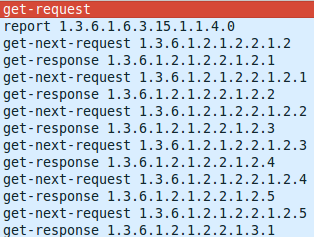
\includegraphics[scale=0.75]{images/snmp/snmpMensajes.png}
	
	\textit{Consulta snmpwalk}
\end{center}

\begin{center}
	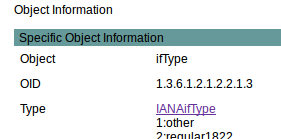
\includegraphics[scale=0.75]{images/snmp/iftypeother.png}
\end{center}


\begin{center}
	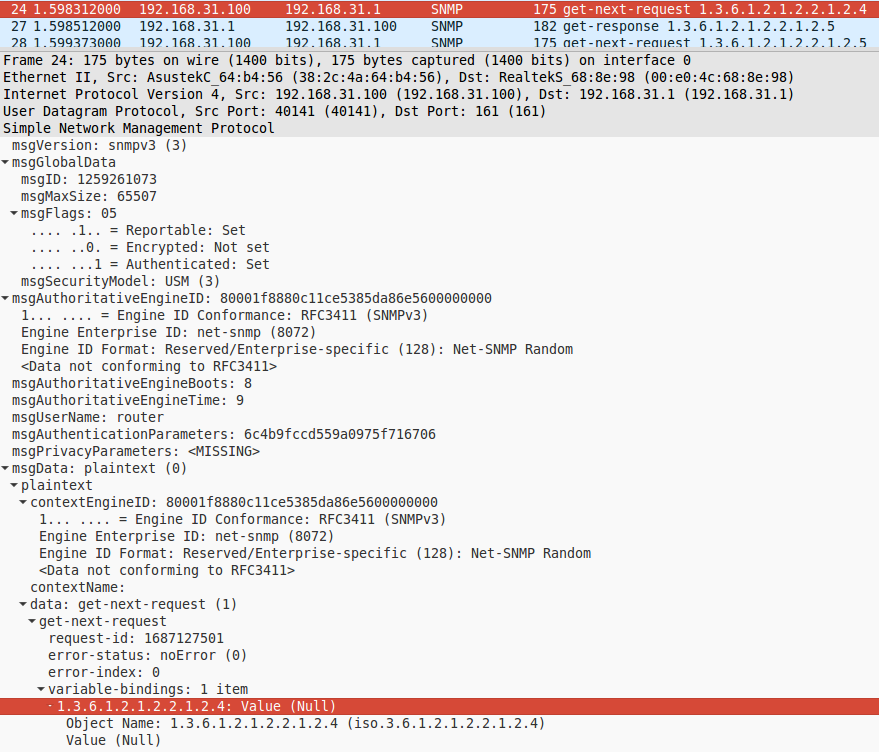
\includegraphics[scale=0.45]{images/snmp/get-next-request.png}
	
	\textit{Mensaje get-next-request preguntando por la quinta interfaz}
\end{center}


\begin{center}
	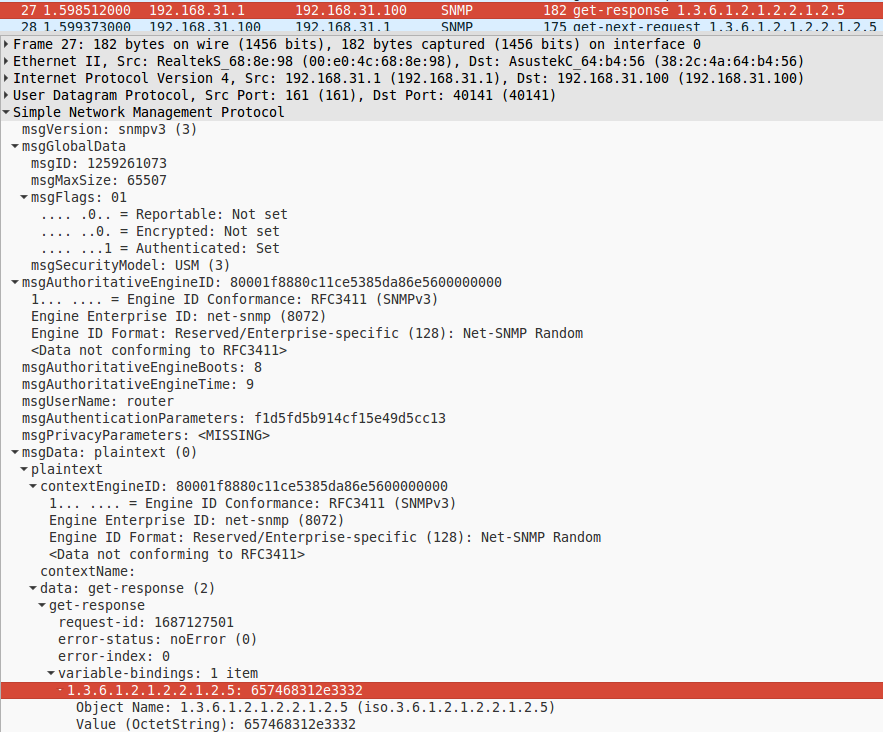
\includegraphics[scale=0.45]{images/snmp/get-response.png}
	
	\textit{Mensaje get-response con la descripción de la quinta interfaz}
\end{center}

\begin{center}
	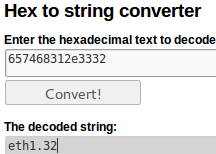
\includegraphics[scale=0.75]{images/snmp/octet.png}
	
	\textit{Valor de la quinta interfaz de HEX a texto}
\end{center}


\subsection{Voz sobre IP}
En esta sección documentamos las configuraciones que hemos tomado para el servidor de Asterisk.

\subsubsection{Configuración básica}
Para las organizaciones 31 y 32, hacemos 2 cuentas de cliente para ambas organizaciones (311 y 312 para organización 31; 321 y 322 para la organización 32).

\begin{Verbatim}
; Organizacion 1
[cliente-311]
type=friend
secret=12345
nat=no
host=dynamic
context=default

[cliente-312]
type=friend
secret=12345
nat=no
host=dynamic
context=default

; Organizacion 2
[cliente-321]
type=friend
secret=12345
nat=no
host=dynamic
context=default

[cliente-322]
type=friend
secret=12345
nat=no
host=dynamic
context=default
\end{Verbatim}

Al establecer el \textit{type=friend} y el \textit{host=dynamic} indicamos que el usuario puede registrarse desde cualquier ip y que se le permite hacer llamadas. Además, todos los usuarios tienen la misma contraseña: 12345.

\hfill

Para esos clientes también hemos configurado sus extensiones.

\begin{Verbatim}
exten => 311,1,Dial(SIP/cliente-311)
exten => 312,1,Dial(SIP/cliente-312)

exten => 321,1,Dial(SIP/cliente-321)
exten => 322,1,Dial(SIP/cliente-322)
\end{Verbatim}

Aquí se declara la extensión telefónica asociada a cada cliente. Para hacerlo sencillo, al cliente 2 de la organización 3.1, se le ha establecido la extensión 312, y siguiendo la misma lógica para los otros tres clientes.

\subsubsection{Troncales Asterisk}
Para empezar, hacemos una redirección básica entre los dos servicios Asterisk en las configuraciones de extensión de Asterisk:
\begin{Verbatim}
[Organizacion-32]
type=friend
host=192.168.32.100
context=default
allow=all
nat=no
insecure=invite
\end{Verbatim}

Arriba se está definiendo la organización 3.2 (esta es la configuración de la organización 3.1). Al establecer \textit{type=friend} y la ip del host así como \textit{allow=all} se permite que la organización 3.2 haga llamadas a clientes de la organización 3.1.

\begin{Verbatim}
exten => _32X,1,Dial(SIP/${EXTEN}@192.168.32.100)
exten => _32X,n,Hangup()
\end{Verbatim}

Por último, con estas dos extensiones se redirigen llamadas con la extensión 32X siendo X cualquier cosa, hacia la organización 32.

La configuración en la organización 3.1 es simétrica, cambiando 192.168.32.100 por 192.168.31.100 y cambiando \textit{\_32X} por \textit{\_31X}.

\subsubsection{Seguridad IPsec}
%DONE

Para proteger la comunicación entre las centralitas de las organizaciones 31 y 32 aplicamos protección por IPsec entre las direcciones de las centralitas, gracias a que elegimos \textit{directmedia=no}, sabemos que cualquier comunicación externa pasará por la centralita y estará protegida. Como en la configuración de la centralita sólo permitimos llamadas en la organización y sólo sabemos redirigir a la organización 31 o 32, también sabemos que no habrá llamadas externas sin proteger.

Sin embargo, en la topología ideal, la aplicación de IPsec se haría en las comunicaciones entre los routers, protegiendo así no sólo el servicio VoIP, sino todas las comunicaciones entre las organizaciones. Como sólo tenemos un router, en la práctica IPsec se instala entre cada servidor de las organizaciones, y para poder analizar los mensajes, no usamos ESP, sólo AH.

Además, en la solución ideal, en caso de que aceptemos llamadas entre otras organizaciones además de la 31 y 32, añadiríamos seguridad TLS o DTLS para UDP, entre la centralita y el otro extremo. En nuestra práctica con IPsec es más que suficiente, y al tener todos los servicios en la misma máquina, todos se benefician como si fuera IPsec entre los routers.

\hfill

La instalación de IPsec se puede seguir en las diapositivas de Servicios Telemáticos del año pasado. Basta con modificar \textit{/etc/ipsec-tools.conf} en ambas máquinas añadiendo para AH, en la máquina de la organización 31:

\begin{Verbatim}[frame=single]
add 192.168.31.100 192.168.32.100 ah 0x200 -A hmac-md5 0xc0291ff014dccdd03874d9e8e4cdf3e6;
add 192.168.32.100 192.168.31.100 ah 0x300 -A hmac-md5 0x96358c90783bbfa3d7b196ceabe0536b;

spdadd 192.168.31.100 192.168.32.100 any -P out ipsec ah/transport//require;
spdadd 192.168.32.100 192.168.31.100 any -P in ipsec ah/transport//require;
\end{Verbatim}


O en caso de poner ESP, en la organización 31:

\begin{Verbatim}[frame=single]
add 192.168.31.100 192.168.32.100 esp 0x201 -E 3des-cbc
 0x7aeaca3f87d060a12f4a4487d5a5c3355920fae69a96c831 -A hmac-md5 0xc0291ff014dccdd03874d9e8e4cdf3e6;
add 192.168.32.100 192.168.31.100 esp 0x301 -E 3des-cbc
 0xf6ddb555acfd9d77b03ea3843f2653255afe8eb5573965df -A hmac-md5 0x96358c90783bbfa3d7b196ceabe0536b;

spdadd 192.168.31.100 192.168.32.100 any -P out ipsec esp/transport//require;
spdadd 192.168.32.100 192.168.31.100 any -P in ipsec esp/transport//require;
\end{Verbatim}

Para la organización 32 es igual cambiando los out por in, y viceversa.

\hfill
\\


Y con un simple ping desde una máquina a la otra podemos ver cómo se añaden las cabeceras AH a los paquetes, en la \autoref{fig:pingreqAH} vemos el ping request y que el campo AH SPI corresponde al 0x200 de la configuración, y en la \autoref{fig:pingreplyAH} del ping reply, el valor es el 0x300 de las comunicaciones desde 192.168.32.100 a 192.168.31.100.


\begin{figure}[h!]
	\caption{Ping Request AH}
	\centering
	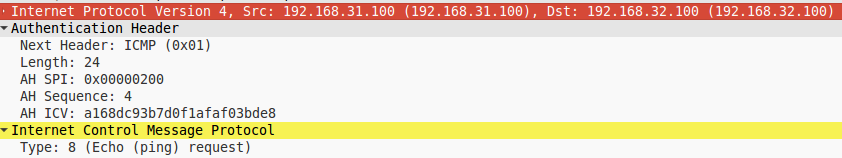
\includegraphics[scale=0.5]{images/ipsec/pingreqAH.png}
	\label{fig:pingreqAH}
\end{figure}

\begin{figure}[h!]
	\caption{Ping Reply AH}
	\centering
	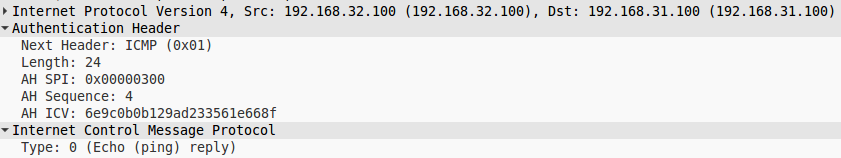
\includegraphics[scale=0.5]{images/ipsec/pingreplyAH.png}
	\label{fig:pingreplyAH}
\end{figure}


\subsubsection{Buzón de voz}
Después de un intento de llamada, a los 5 segundos salta el buzón de voz. Los clientes después pueden comprobar su buzón de voz llamando al 123.

\begin{Verbatim}
; Primero se intenta llamar (5 segundos), y después buzón de voz (VoiceMail).
exten => 311,1,Dial(SIP/cliente-311,5)
exten => 311,n,VoiceMail(311@vm-org31,u)
exten => 312,1,Dial(SIP/cliente-312,5)
exten => 312,n,VoiceMail(312@vm-org31,u)

; Llamando al 123 se puede acceder al buzón de voz.
exten => 123,1,Answer(500)
exten => 123,2,VoiceMailMain(@vm-org31)
\end{Verbatim}

\subsubsection{Análisis de trazas}

El registro de un cliente en la plataforma en 4 paquetes:

\begin{center}
	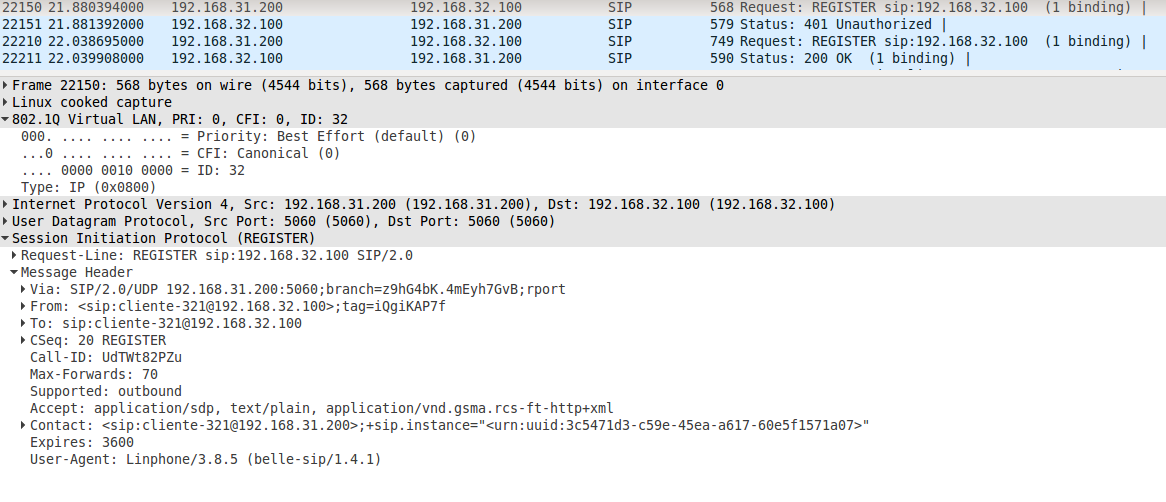
\includegraphics[width=1\linewidth]{images/voip1}
\end{center}

Intento de registro. Se indica la procedencia y el user-agent así como el identificador del cliente.

\begin{center}
	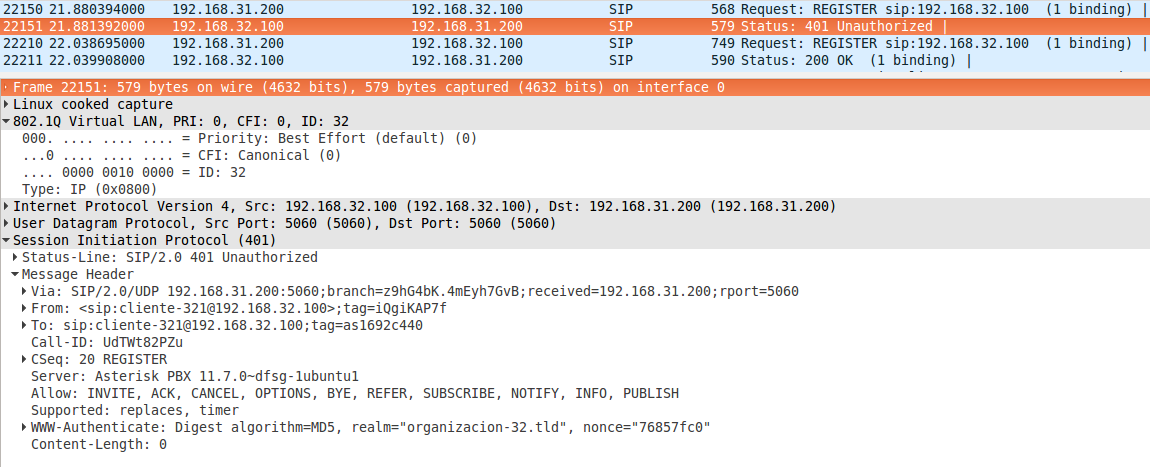
\includegraphics[width=1\linewidth]{images/voip2}
\end{center}

El servidor responde indicando que para conseguir el registro debe autenticarse. Para ello debe proteger la contraseña usando MD5 y el nonce indicado.

\begin{center}
	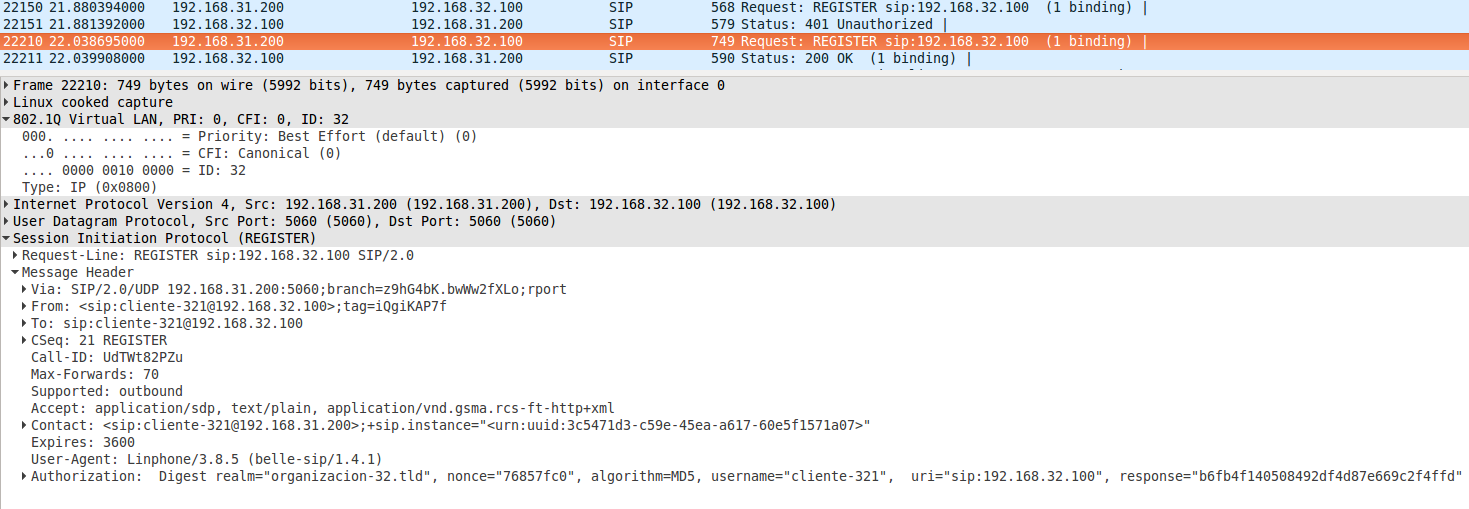
\includegraphics[width=1\linewidth]{images/voip3}
\end{center}

Paquete muy parecido al primero, solo que este lleva en la cabecera la opción \textit{Authorization}, con el \textit{response} al $MD5(nonce+password)$.

\begin{center}
	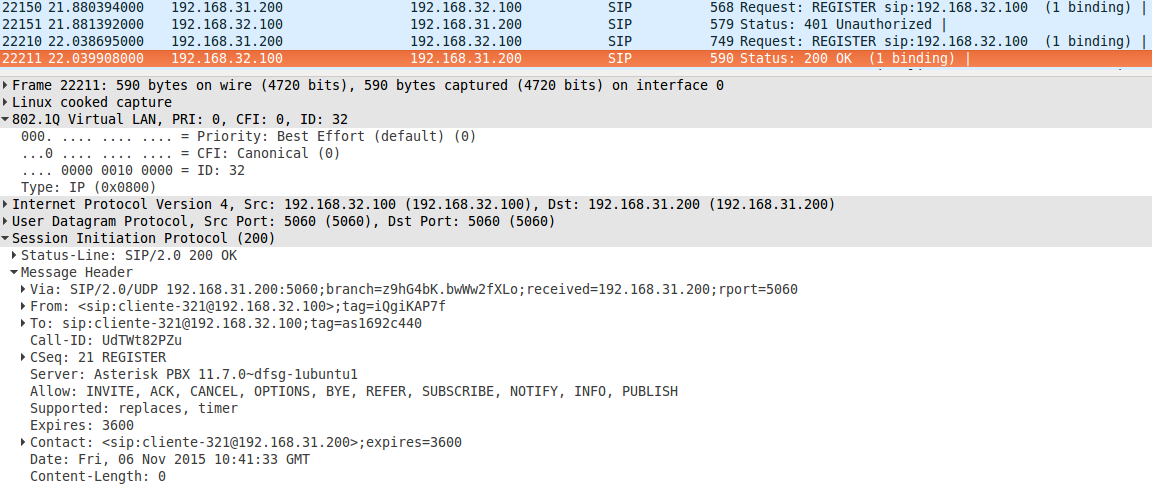
\includegraphics[width=1\linewidth]{images/voip4}
\end{center}

El servicio Asterix autoriza al cliente-321 desde la ip 192.168.31.200, y se lo comunica mediante un \textbf{OK 200}.

\subsection{LDAP}
El servicio LDAP ofrece al resto de servicios un punto en común donde encontrar la información relevante de los usuarios (nombres,organización a la que pertenecen, permisos de uso y acceso, credenciales, etc).

Como contiene la información crítica de los usuarios que se integran en los servicios, LDAP se despliega en su propia máquina.

Sin embargo, en el despliegue real del laboratorio, LDAP está integrado en el ordenador de la organización 31.

Para las pruebas de laboratorio, la instalación y la configuración la generamos automáticamente (sin necesidad de interacción del administrador), en python, generando tres clientes de la organización 31.

Estos tres clientes se generan con el servicio Owncloud en mente. Para organizar la pertenencia de usuarios de Owncloud en el árbol, hemos decidido usar el campo Organizational Unit con valor \textit{owncloud} para indicar la pertenencia al servicio.
                                                                                                                                                                                                                                                                    
Este caso es el más sencillo para aplicar en nuestro caso práctico, pero no es el mejor para la topología ideal. El servicio ldap no lo suele usar un único servicio, y no todos los usuarios tienen acceso a los mismos servicios en una organización. Por ejemplo, el servicio Golum de la Universidad de Murcia frente al de correo o UmuBox.

La solución ideal sería tener los usuarios registrados sin indicar los servicios por la \textit{ou}, sino crear un grupo por cada servicio, y del que cuelguen identificadores de los usuarios que pertenecen al grupo. Así, un usuario registrado en ldap tiene una sola entrada con todos sus datos, y cuelga de una sola \textit{ou}, no de varias posibles, y para asignarle a un servicio, sólo hay que ir al nodo del servicio y dar de alta la hoja del usuario.

Ejemplo de entrada ldap: \textit{cliente311.ldif}:

\begin{BVerbatim}
# Entrada para los usuarios:
dn: cn=cliente311, ou=owncloud, dc=org31, dc=es
changetype: add
objectclass: inetOrgPerson
sn:Perez
cn: cliente311cn
uid: cliente311uid
userPassword: manyhue
ou:owncloud
\end{BVerbatim}

%TODO: Indicar puertos usados.
%TODO: hacer consulta entre organizaciones, con un ldapsearch más simple

A continuación se muestran imágenes de la traza capturada durante la orden: \textit{ldapsearch -x -b “dc=org11,dc=es"\ “ou=owncloud"\ dn description}:

Las dos primeras trazas indican el acceso a ldap. Las dos últimas indican que la búsqueda ha terminado con éxito y que se puede terminar la consulta.

\begin{center}
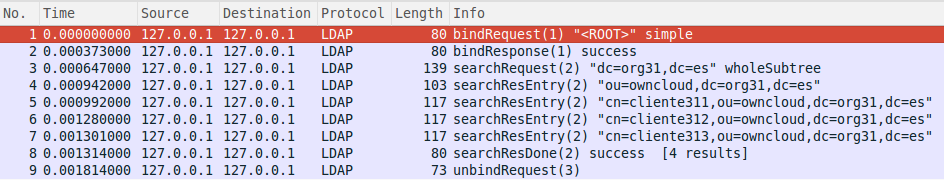
\includegraphics[scale=0.5]{images/ldap/ldap1}
\end{center}

Aquí se muestra la tercera traza con la petición de búsqueda del comando, con el objeto \textit{“dc=org11,dc=es"} como punto inicial de búsqueda, el filtro de \textit{“ou=owncloud"} y los atributos a devolver \textit{dn} y \textit{description}.

\begin{center}
	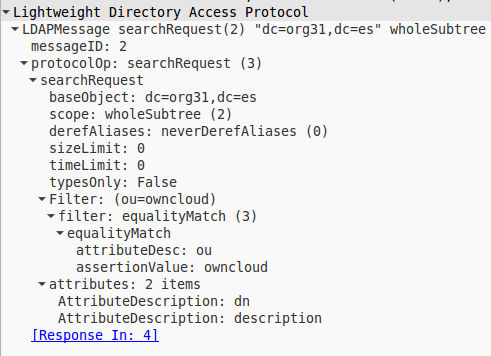
\includegraphics[scale=0.5]{images/ldap/ldap2}
\end{center}

Las siguientes imágenes muestran los resultados (\textit{searchResEntry}), con la entrada que define la propia O.U. Owncloud, seguido de las entradas de los clientes \textit{cliente311}, \textit{cliente312} y \textit{cliente313}.

\begin{center}
	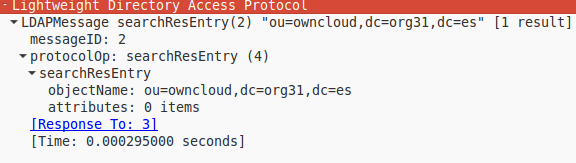
\includegraphics[scale=0.5]{images/ldap/ldap3}
\end{center}
\begin{center}
	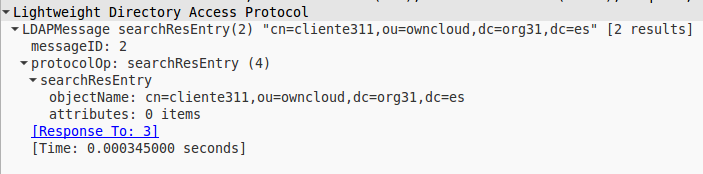
\includegraphics[scale=0.5]{images/ldap/ldap4}
\end{center}
\begin{center}
	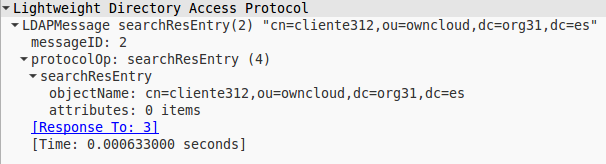
\includegraphics[scale=0.5]{images/ldap/ldap5}
\end{center}

\begin{center}
	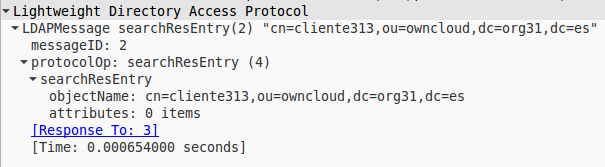
\includegraphics[scale=0.5]{images/ldap/ldap6}
\end{center}


\subsection{OwnCloud}
%TODO
\section{Políticas de seguridad}
Para las políticas de seguridad nos centramos en explicar la organización 1, ya que la organización solo tiene que proteger VOIP y se haría de manera simétrica a la organización 1.

\begin{center}
	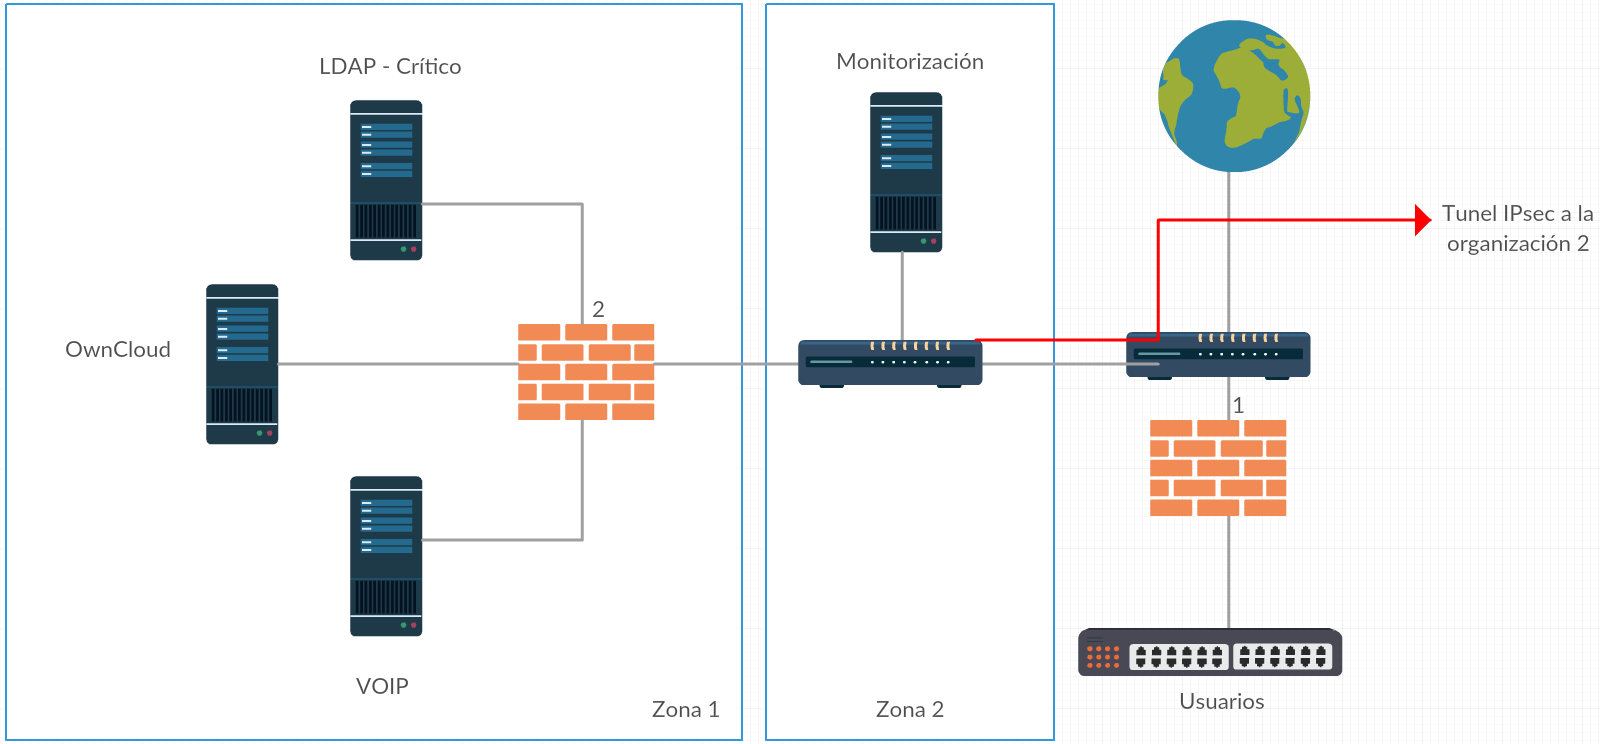
\includegraphics[width=1\linewidth]{images/seguridadorg1}
\end{center}

A las zonas 1 y 2 solo deberá entrar el administrador y deberá estar protegida de cualquier acceso físico. En caso de que no funcione el servidor de LDAP se instalará una copia de seguridad en el servidor de OwnCloud, y se repondrá con un servidor nuevo lo antes posible.

Si falla el servidor de VOIP o el de OwnCloud, se instalará una copia de seguridad en el otro servidor (nunca en el de LDAP), y se repondrá con otro servidor nuevo cuanto antes.

Si el servidor de monitorización deja de funcionar, se permitirá el acceso a un usuario a las zonas 1 y 2 bajo previo aviso del administrador y con el único objetivo de establecer una manera de acceder por SSH a los servicios de forma temporal (ya que el servidor de monitorización es el único que permite hacer el puente SSH entre el exterior y los servicios).

\subsection{Análisis de riesgos}
El escenario tiene como servicios a proteger:

\begin{itemize}
	\item LDAP
	\item OwnCloud
	\item Voz sobre ip
	\item SNMP + Nagios3
\end{itemize}

De estos servicios los únicos que tienen que ofrecer funcionalidad al exterior son OwnCloud (que está localizado en la organización 31) y VOIP (con dos servidores dedicados ASTERIX, uno en cada organización).

Por lo tanto, los otros dos servicios (SNMP y LDAP) hay que protegerlos completamente de accesos al exterior. 

Como LDAP es un servicio crítico (contiene el directorio de usuarios, y se usa para otros servicios), en un escenario real LDAP estaría en su propia máquina con todo capado salvo el acceso desde el servidor OwnCloud que necesita acceso para los usuarios registrados.

La máquina con la etiqueta monitorización haría de centro de control. Sería la única con acceso ssh al exterior y la única desde la cual se puede hacer ssh al resto de servidores (y al router), además de monitorizar todos los dispositivos con Nagios y SNMP.

En este escenario, para poder manipular remotamente el servicio LDAP por ejemplo se necesitaría acceder al servidor de monitorización y después al de LDAP, duplicando la seguridad. En caso de que el servidor de monitorización estuviera comprometido, todavía haría falta un nivel más de acceso para poder llegar a los servicios de la zona 1.

Por lo tanto el firewall 2 permitiría:

\begin{itemize}
	\item LDAP solo hacia OwnCloud: TCP puerto 389 entre las máquinas OwnCloud y LDAP
	\item OwnCloud hacia el exterior: TCP puerto 443 desde cualquier lugar
	\item VoIP hacia el exterior: UDP 5060 para sip y UDP 10000 al 20000 para RTP hacia cualquier lugar
	\item SSH solo hacia la zona 2: TCP puerto 22 entre cualquiera de las máquinas de servicios y la máquina de monitorización.
\end{itemize}

Además, toda conexión Asterix entre ambas organizaciones viajaría por IPsec una vez cruzado el firewall 2.

\subsection{Configuración de seguridad}
Las iptables no se corresponden con la expliación anterior pues la infraestructura real del laboratorio 2.7 no coincide a la ideal. Aquí solo hay un cortafuegos que se establece en el router y que protege a la vez a usuarios y a ambas organizaciones:

\lstinputlisting{../iptables}

\subsection{Generación de certificados}
%DONE

La creación de una jerarquía de certificados con su CA no se establece como un servicio a desplegar para el público o clientes, pero lo necesitamos en esta práctica de cara a la seguridad TLS de Owncloud.

En el caso ideal de nuestra organización, de ofrecer el servicio de nuestra CA para firmar solicitudes de certificados dispondríamos una máquina física en la red DMZ cuya única función sea la de almacenar la clave privada de la CA, firmar las solicitudes y por supuesto generar las lístas de CRL publicándolas en el servidor web. Esta máquina es tan crítica en la seguridad que dispondría de un firewall que la aislara del tráfico de la red DMZ como una segunda capa de seguridad, donde sólo se permitan comunicaciones desde el servidor para el intercambio de ficheros criptográficos, y el servidor HTTP/S donde registrarse por primera vez.

Siguiendo el ejemplo de otras CA, el procedimiento para firmar un certificado de un servidor web sería: el cliente registra el dominio que quiere que se certifique, se le indica que instale un script en el servidor, el cual escuchará las conexiones proactivas del servidor de la CA, que hará una comprobación con datos aleatorios para comprobar que es la máquina del dominio indicado y el script instalado, se le indica al script que genere el par de claves y el csr, se envía responde a la CA con el csr y ésta termina devolviendo el certificado público firmado. De esta manera, la única comunicación que recibiría la CA sería la dirección del servidor, y el resto de comunicaciones las iniciaría la máquina de la CA. Es más, el servidor web sería el que dispusiera el formulario de registro y la única máquina que el nuevo firewall permitiera comunicarse con el servidor de la CA.

Para administración, el firewall añadiría un acceso por ssh desde una máquina específica de un administrador del sistema desde la red interna a la organización, y por una VLAN reservada exclusivamente para dicho propósito.

Teniendo en cuenta que tratamos con la clave privada de nuestra CA, nunca se es demasiado paranoico.


\hfill


En nuestro caso práctico, las claves de la CA para generar los CRL se encuentra en la misma máquina que el resto de servicios (nada recomendable), y para generar las claves seguimos los pasos de las diapositivas de prácticas, añadiendo los siguientes detalles:

\begin{itemize}
	\item En el fichero \textit{openssl.conf} en la sección $[$ usr\_cert $]$, la que indica qué hay que hacer al firmar una solicitud csr, hay que añadir la línea \textit{crlDistributionPoints = URI:http://server.org31/crl/org31.CRL} para indicar, en los certificados firmados, que la CA generará las listas de CRL y las publicará en la dirección \textit{http://server.org31/crl/org31.CRL}, que en nuestro caso es el mismo servidor apache2 que Owncloud.
	\item El certificado del servidor hay que darle como \textit{common name} \textit{server.org31}, que es el nombre por el que accederemos desde el navegador, el escrito en \textit{/etc/hosts} a falta de servidor DNS.
	\item Con crontab añadimos el comando de generar una nueva lista actualizada de los CRL a las doce de la noche cada día, copiándola en el servidor web indicado antes.
	\item Al servidor apache2, en la configuración de SSL se le debe indicar dónde está su certificado, que compruebe el certificado de los clientes y haga una comprobación de los certificados revocados por la lista CRL.
	\subitem Para la comprobación de CRL se debe indicar un fichero (o una carpeta con ficheros nombrados por hash) donde se encuentre un fichero CRL correcto.
	\subitem Entre los problemas que nos hemos ido encontrando en el despliegue, se encuentra que Apache no comprueba la lista de CRL indicada con la extensión del primer punto, sino que siempre compara con el fichero indicado, y en caso de modificar el fichero, se debe reiniciar el servicio. Por ello, para las pruebas de revocación, se copia `forzosamente' el CRL actualizado en el fichero de Apache, aunque se siga publicando en la dirección web.
\end{itemize}

\hfill

Para las pruebas, tenemos el certificado de la CA, el de \textit{server.org31} y el de \textit{cliente}, no necesitamos más en las pruebas, pues sólo tenemos un servidor y el certificado de cliente es para comprobar la revocación, no hemos añadido que sirva para iniciar sesión en Owncloud en vez de escribir usuario y contraseña.

Primero comprobamos que sin el certificado el servidor no nos deja acceder a Owncloud por HTTPS en la \autoref{fig:pedircert}, después, que con el certificado del cliente, \autoref{fig:usercert1} y \autoref{fig:usercert2}, sin revocar nos permite acceder,  \autoref{fig:https}, y finalmente revocamos el certificado de \textit{cliente}, actualizamos el CRL, lo copiamos en el fichero de Apache, reiniciamos el servidor, y volvemos a intentar acceder, recibiendo un error por la revocación del certificado, en \autoref{fig:revoked}.


\begin{figure}[h]
	\caption{Petición certificado de cliente}
	\centering
	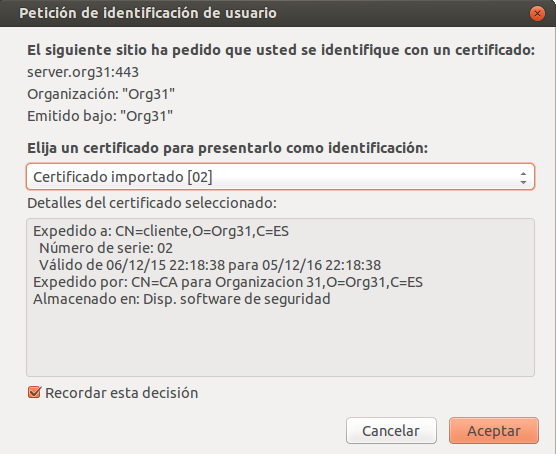
\includegraphics[scale=0.5]{images/certs/pedircert.png}
	\label{fig:pedircert}
\end{figure}


\begin{figure}[h]
	\caption{Conexión HTTPS}
	\centering
	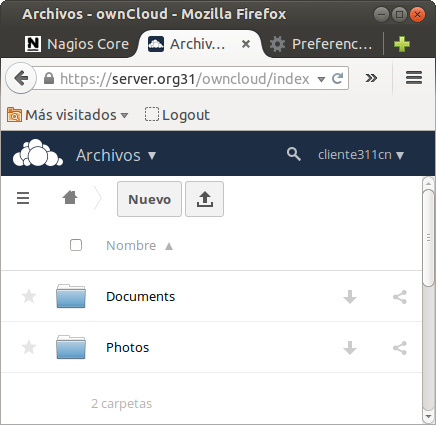
\includegraphics[scale=0.5]{images/certs/https.png}
	\label{fig:https}
\end{figure}

\begin{figure}[h]
	\caption{Certificado de usuario 1/2}
	\centering
	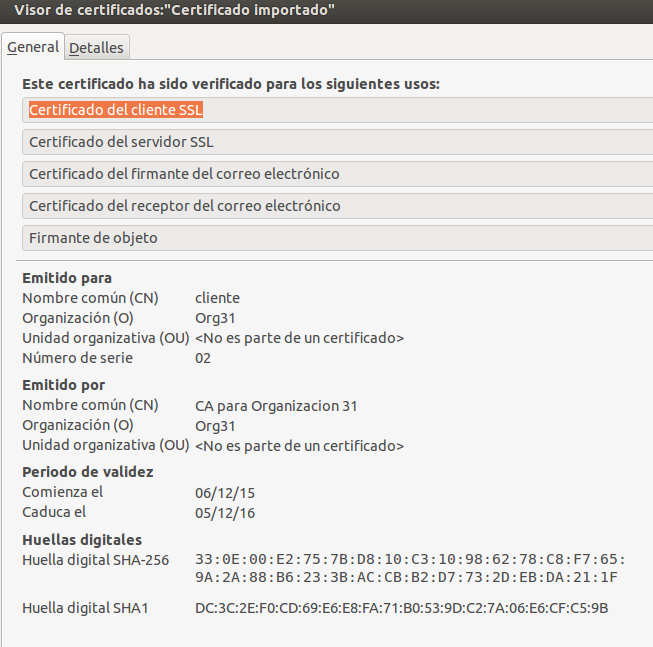
\includegraphics[scale=0.5]{images/certs/usercert1.png}
	\label{fig:usercert1}
\end{figure}


\begin{figure}[h]
	\caption{Certificado de usuario 2/2}
	\centering
	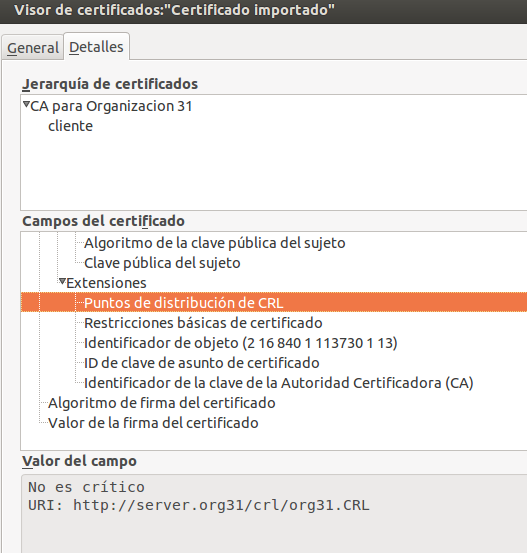
\includegraphics[scale=0.5]{images/certs/usercert2.png}
	\label{fig:usercert2}
\end{figure}

\begin{figure}[h]
	\caption{Certificado del servidor}
	\centering
	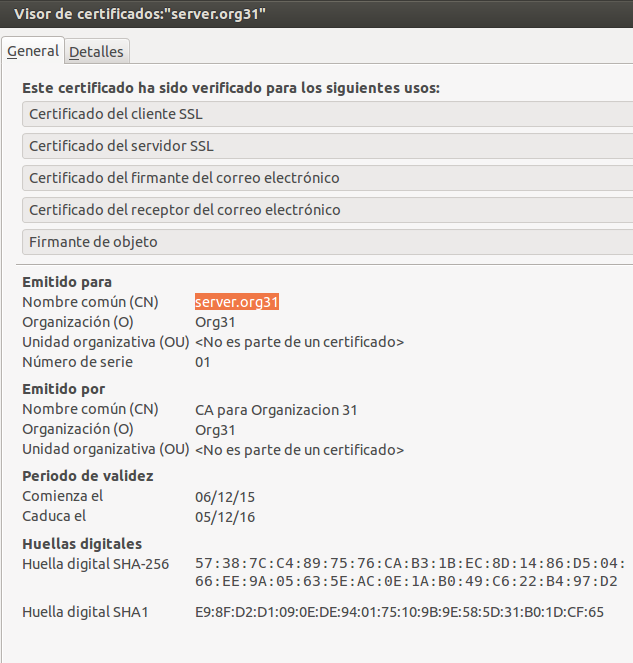
\includegraphics[scale=0.5]{images/certs/servercert1.png}
	\label{fig:servercert1}
\end{figure}

\begin{figure}[h]
	Revocación del certificado de \textit{cliente}:
\begin{Verbatim}[frame=single]
alumno@Laboratorio27:~/demoCA$ openssl crl -in /var/www/crl/org31.CRL -text -noout 
	Certificate Revocation List (CRL):
		Version 2 (0x1)
	Signature Algorithm: sha256WithRSAEncryption
		Issuer: /C=ES/O=Org31/CN=CA para Organizacion 31
		Last Update: Dec 14 18:29:43 2015 GMT
		Next Update: Jan 13 18:29:43 2016 GMT
		CRL extensions:
			X509v3 CRL Number: 
				2
	Revoked Certificates:
		Serial Number: 02
	Revocation Date: Dec 14 18:28:56 2015 GMT
	Signature Algorithm: sha256WithRSAEncryption
		a7:a6:7d:75:92:81:4f:e1:21:b4:db:58:5b:60:dd:b8:12:0c:
		9f:83:53:d0:41:59:34:2c:d1:e4:d2:56:a9:ce:01:b5:8e:4f:
		53:0f:f4:40:1c:95:d6:55:77:9f:82:a2:d1:fc:b4:07:dd:46:
		d0:bd:d3:47:c3:46:7a:cb:af:e6:09:86:55:68:eb:dd:f2:8b:
		19:a0:91:d5:5c:d2:e7:1e:7f:38:a1:31:de:6a:2e:e6:cb:d5:
		fa:af:02:33:12:34:47:22:8a:41:da:ff:96:bb:ca:52:72:b9:
		11:97:e7:20:46:44:e5:13:5d:9d:5a:da:34:71:d4:09:87:f4:
		7a:2d:d5:6c:d6:ea:b0:6b:4e:db:28:f4:c9:81:ef:b1:16:43:
		50:b7:be:9e:e6:95:af:60:ce:8f:ad:9c:99:f3:f7:2e:24:5a:
		92:13:03:b4:a8:d8:e9:e2:05:b7:89:95:d0:07:88:d4:d8:99:
		bd:5f:2c:35:8c:18:90:d9:d3:93:80:db:ea:4f:e6:83:d1:7c:
		b2:83:ce:fb:c5:6b:3c:15:af:bb:31:1b:42:7e:44:44:b5:d8:
		a3:ca:fd:0e:0c:ac:ab:b5:b0:47:8e:00:65:cd:e1:d0:e2:5b:
		5d:55:5e:d8:43:96:8d:cc:55:6c:ee:a0:3b:c0:bb:b7:80:bc:
		3c:ec:30:c2
\end{Verbatim}
\end{figure}


\begin{figure}[h]
	\caption{Certificado de cliente revocado}
	\centering
	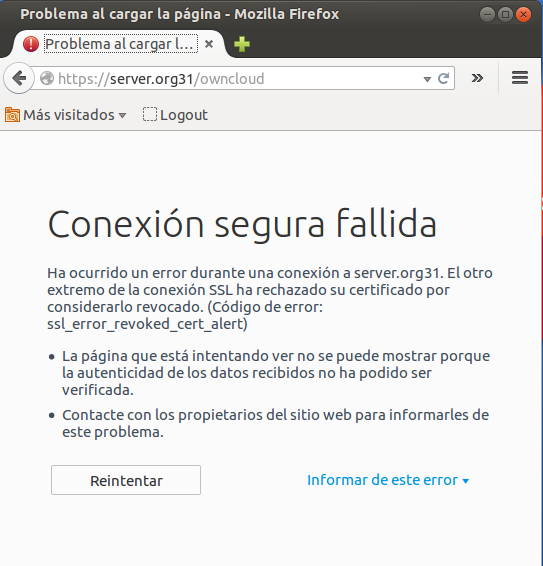
\includegraphics[scale=0.5]{images/certs/revoked.png}
	\label{fig:revoked}
\end{figure}



\section{Conclusiones}

Tras estos casi cuatro meses de práctica, nuestras impresiones finales son que su principal propósito es que los alumnos investiguemos por nuestra cuenta y nos enfrentemos a los problemas reales que supone un despliegue de este tipo. En cualquier \textit{tutorial} puedes leerte los pasos y pensar que eso funcionará a la primera, pero lo importante son los fallos inesperados, que aunque te lleven uno o dos días solucionarlos, ese trabajo no forma realmente parte del resultado final, no como lo hace añadir una característica nueva, tipo el buzón de voz a Asterisk. Son problemas como descubrir hasta dónde comprueba apache2 un certificado, que la versión de SNMP instalada tiene un fallo en concreto con una orden, que AH en IPsec modifica el campo \textit{protocol} del paquete IP y el protocolo (TCP, UDP, ...) ahora está en \textit{next header}, de modo que iptables no lo tiene en cuenta, ...
               
               
               
Además, por el orden de las prácticas, nosotros propondríamos un cambio donde los certificados fueran lo primero, pues ya se vieron en Servicios Telemáticos, de modo que la siguiente práctica puede empezarse en la misma clase. El servicio SNMP lo pondríamos casi al final de todos, pues cuando lo hemos dado el primero, al principio no se ve qué puedes gestionar realmente. Después de haber desplegado, por ejemplo, Asterisk, si entonces viéramos SNMP, se nos ocurriría que sería útil para controlar que esté el servicio escuchando por UDP o TCP, según lo hayamos configurado en \textit{sip.conf}, etc.

El servicio de iptables no lo tenemos tampoco claro como el último. Estando al final puedes escribir todas las iptables de una vez, aunque luego las pruebes una a una, pero dan problemas y la falta de tiempo se nota. Estando de las primeras prácticas se podrían añadir los servicios mínimos (DNS, conexiones TCP ya establecidas, etc.) al inicio, e ir añadiendo las reglas nuevas necesarias para el nuevo servicio desplegado. Idealmente, de esta forma las iptables se crearían junto a los servicios y no serían de golpe unas decenas de reglas que implementar. Pero aquí se enfrentan el modelo se parece al de SNMP, de darlo lo primero para ir juntándolo con otros servicios, y que iptables sí sería necesario llevarlo al día para que los servicios funcionen.



\end{document}
